\section{Holiday and Sick Leave Detection}

The goal of this attack is to simply detect miss-out and if a contributor has anomalies in their regular work day pattern.

Due to possible fluctuations or changes in work routine, one requirement to this algorithm is the detection of a regular work pattern for a given interval.
It must have the ability to adjust to a changing work pattern, but at the same time it needs to be capable of detecting anomalies in this pattern.

The input for this analysis is the intersection between all commits from the considered repositories and all commits from the considered contributors.
The commits' metadata used for this analysis are timestamps as well as additions and deletions in lines of code.

\begin{figure}[H]
    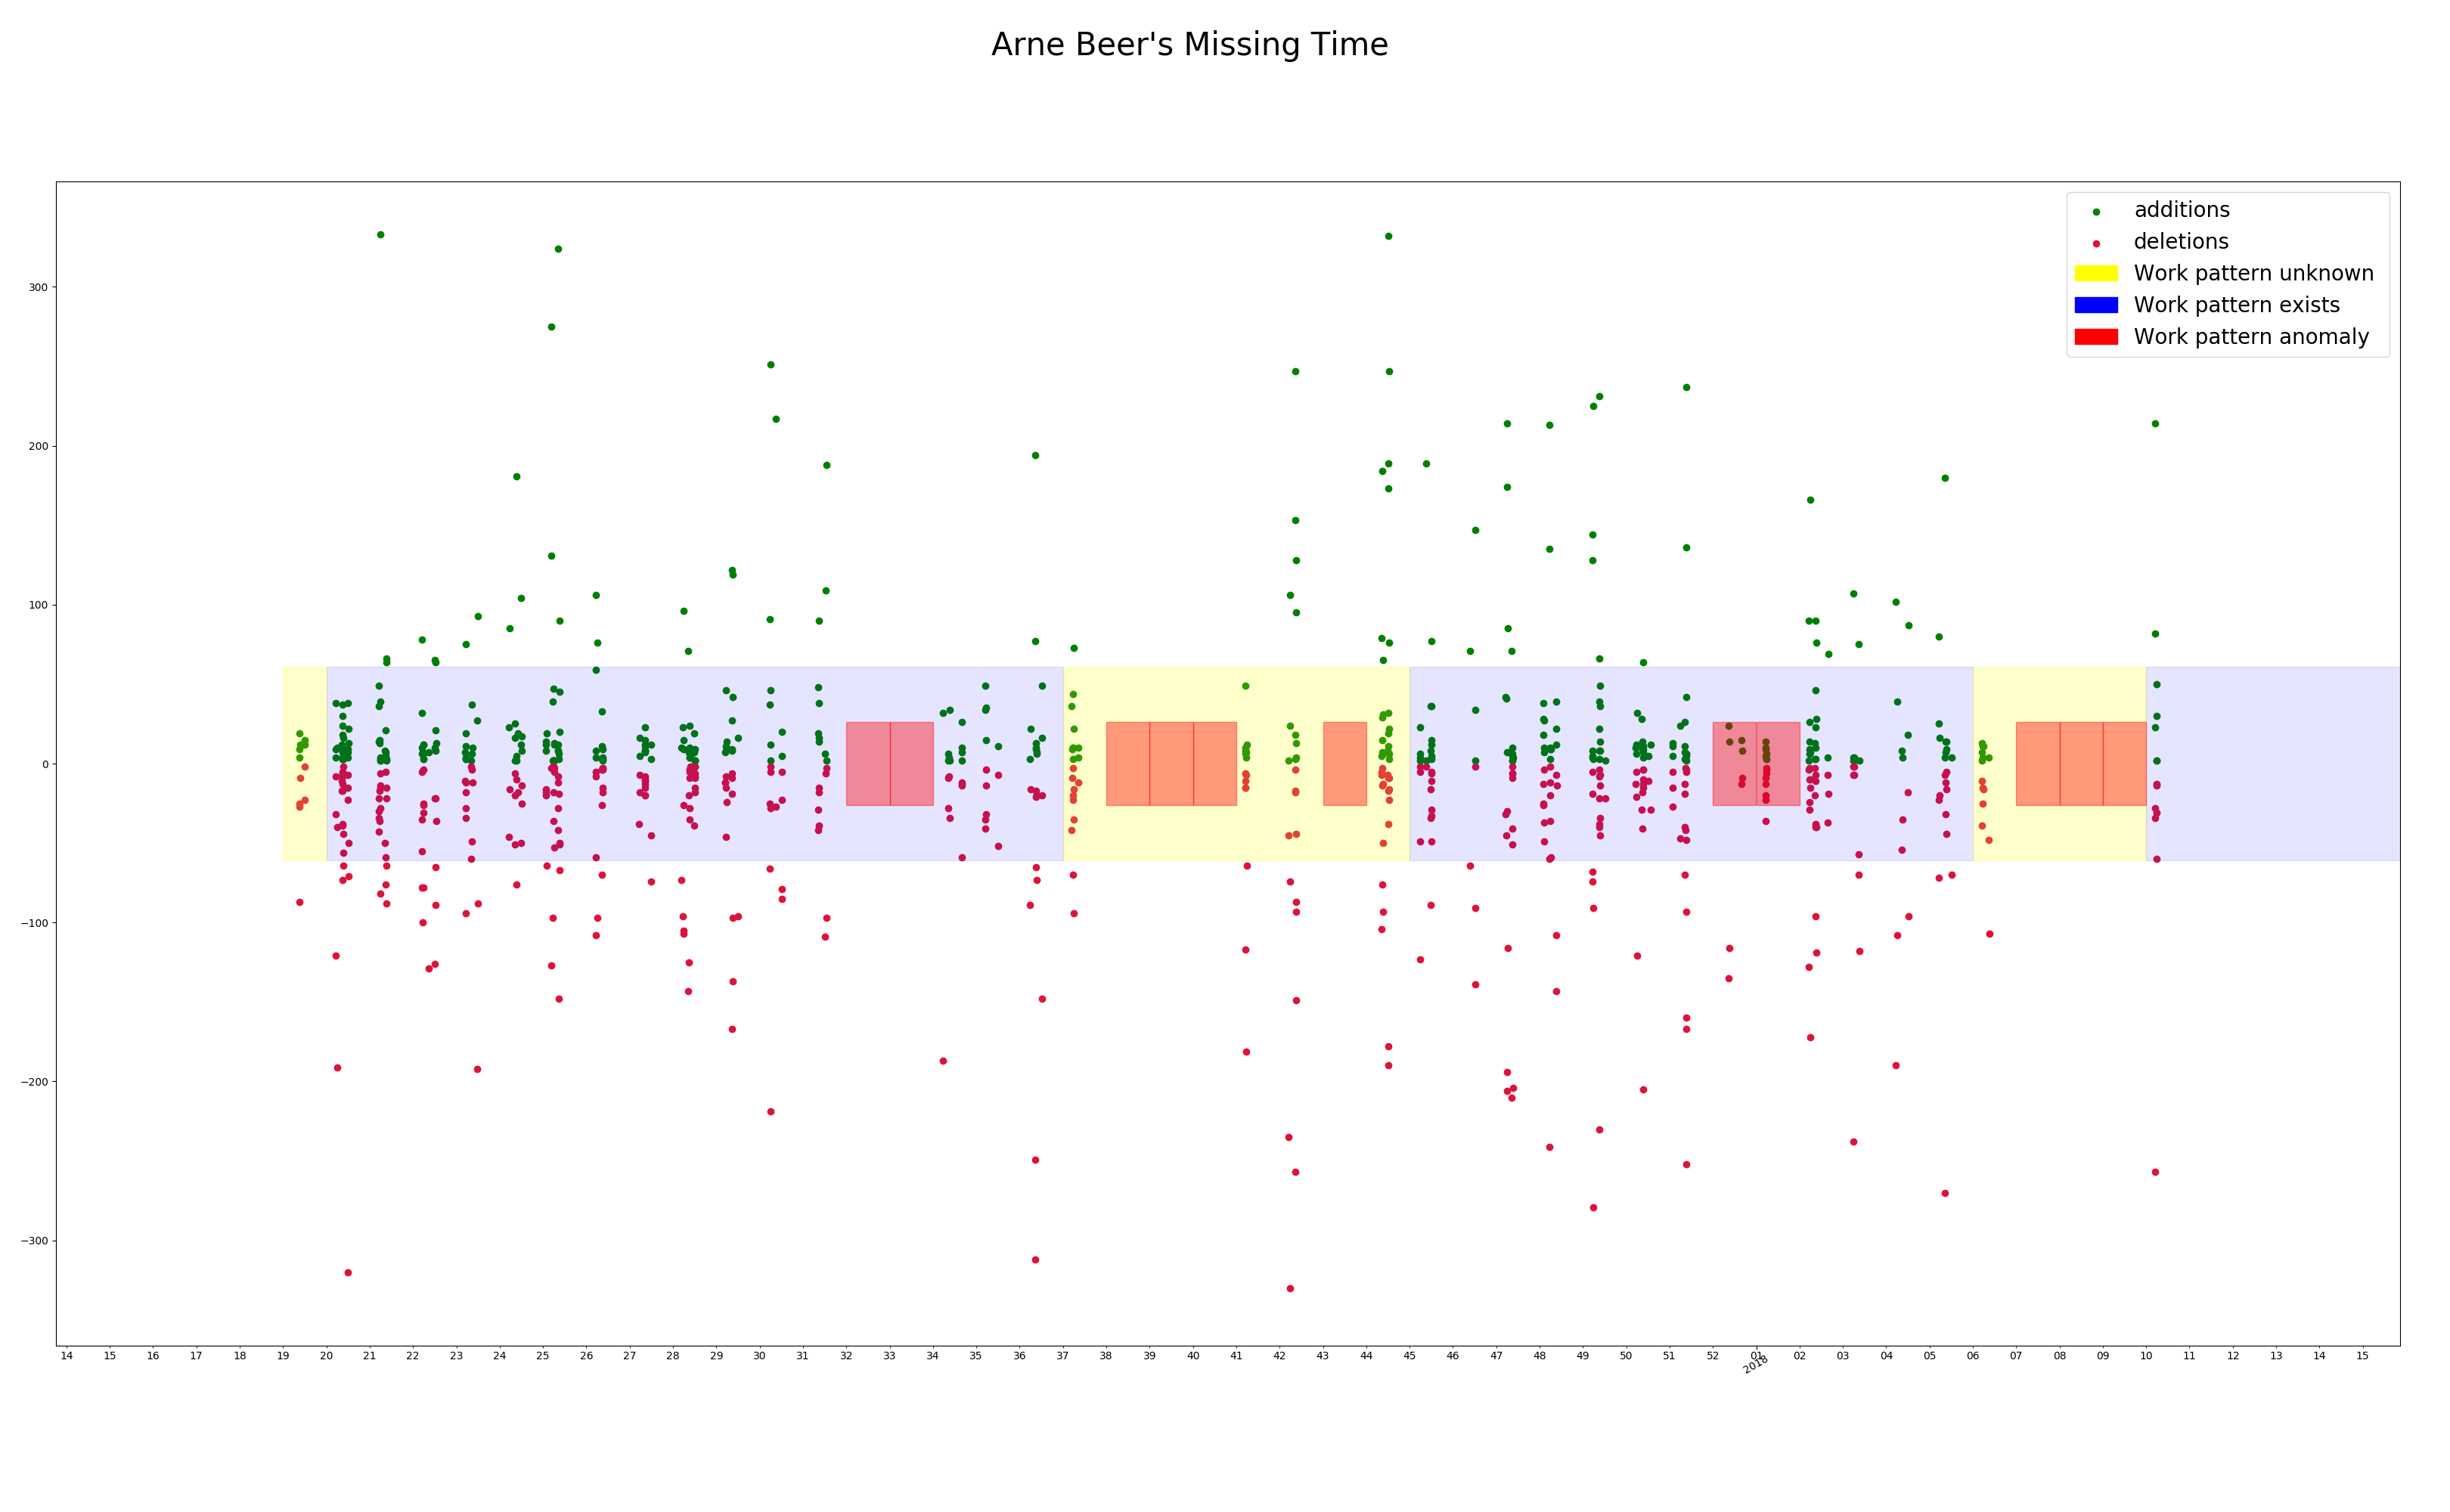
\includegraphics[scale=0.20]{./graphs/analysis/work-time-analysis}
    \centering
    \caption{The work time analysis of an employee.}\label{fig:missing-time}
\end{figure}

The analysis of the data is a chronological scan of all commits for a specific user.
Before performing the actual analysis, the data is converted into an easier to handle format.
It is really difficult to measure productivity in lines of code or in the number of commits made by a person, as they do not necessarily display the amount of work, which has been put into this code.
As a result I decided, that a day counts as a work day as long as at least a single commit is created during the day.
The preprocessed data is thereby equivalent to the days a contributor worked on, ordered by the week of the year.

\begin{minted}[linenos]{python}
def analyse(weeks):
    prototype = None
    for index, week in weeks.items():
        next_six_weeks = weeks[index:index+future_lookup]
        if not prototype:
            # See if there is a prototype in the next few weeks.
            prototype = find_prototype(next_six_weeks)

            # Check if this specific week is a anomaly
            check_anomaly(prototype, week)

            continue

        prototype_exists = prototype_exists_in_next_weeks(next_six_weeks)
        if not prototype_exists:
            # We couldn't find the prototype in the next few rows
            # Try to find a new prototype
            prototype = find_prototype(next_six_weeks)

        check_anomaly(prototype, week)


def check_anomaly(prototype, week):
    if week.working_days == 0:
        save_anomaly(week)

    if prototype is not None:
        different_days = week.working_days - prototype.working_days
        // A single day variance is acceptable
        if different_days >= 1:
            save_anomaly(week)

\end{minted}
\begingroup
\captionof{listing}{Miss-out analysis algorithm.}\label{lst:miss-out-algorithm}
\endgroup

The algorithm inspects every week work pattern of a given interval, which has been set to a year for this analysis.
At the beginning, a new \emph{prototype} is tried to be found.
This is performed in the function \inlinecode{find\_prototype} in Listing~\ref{lst:miss-out-algorithm}.
A prototype is a representative week work pattern, which resembles the average work day pattern of the next weeks.


\begin{minted}[linenos]{python}
def find_prototype(self, weeks, threshold):
    """Look at the first few weeks to find a new prototype."""
    # Create an entry for each pattern and count the occurrences of this entry
    occurrence_counter = {}
    for _, week in weeks.iterrows():
        pattern = week.pattern
        if pattern not in occurrence_counter:
            occurrence_counter[pattern] = {
                'prototype': week,
                'count': 1,
            }
        else:
            occurrence_counter[pattern]['count'] += 1

    # Get the prototype for the pattern with the most occurrences
    #
    # If there is no week which solely has the most occurences, return None.
    # In this case we can't predict a proper prototype.
    max_count = 0
    invalid = False
    prototype = None
    for _, item in occurrence_counter.items():
        if item['count'] > threshold and item['count'] > max_count:
            prototype = item['prototype']
            max_count = item['count']
            invalid = False
        elif item['count'] == max_count:
            invalid = True

    if invalid:
        return None

    return prototype
\end{minted}
\begingroup
\captionof{listing}{Miss-out analysis algorithm.}\label{lst:prototype-detection}
\endgroup

This function, which can be seen in Listing~\ref{lst:prototype-detection}, performs a simple iteration over a fix amount of future weeks, to find a work day pattern occurring more often than a given threshold.
If a prototype is found, we are capable of identifying anomalies that deviate from this pattern.

For each following week it is then firstly checked if this week is a anomaly in regards to the current prototype.
Anomalies are simply detected by comparing the amount of working days of the prototype and the considered week.
The difference in the working patterns is not suitable for this analysis, as it produces too many false positives for employees with flexible work time.

Secondly it is checked if a week identical to the prototype exists in the near future.
If there is no such week, the current prototype is reset and a new prototype needs to be found again.

In case no prototype can be found, anomalies cannot be easily identified, as there exists no pattern to check against.
Only obvious anomalies, namely weeks without a single work day, will then be marked as such.
